\section{Relations Between Conjectures}

\begin{frame}[label=relations]{Relations}
\begin{mypic}
\begin{scope}[scale=0.75,transform shape]
\tikzstyle{r}=[rectangle,inner sep=1mm,draw,text centered, text width=44mm]

\node[r,text width=28mm] (w) at (5.5,3) {\small Weak Greedy\\ Hierarchical Conjecture\\};
\node[r] (cc) at (0,5) {\small Collapsing Conjecture}; 
\node[r] (gc) at (0,1) {\small Greedy Conjecture};
\node[r] (ghc) at (0,3) {\small Greedy Hierarchical\\ Conjecture\\}; 

\node[r, text width=32mm] (ca) at (10,5) {\small CA is 2-approx};
\node[r, text width=32mm] (gha) at (10,3) {\small GHA is 2-approx};
\node[r, text width=32mm] (ga) at (10,1) {\small GA is 2-approx};

%\draw[help lines] (0,0) grid (14,6);

\foreach \f/\t in {cc/ghc, cc.east/w, ghc/w, gc.east/w, ghc/cc}
  \draw[->] (\f) -- (\t);
  
\foreach \f/\t in {cc/ca, w/gha, gc/ga}
  \draw[dashed,->] (\f) -- (\t);
 
\end{scope}
%\foreach \f/\t in {cc/ca, cc/w, gc/ga, gc/w, w/gha, ga/gha}
 % \draw[->] (\f) -- (\t);
\end{mypic}
\end{frame}

\begin{frame}{Supporting Conjectures}
\begin{itemize}
\item All the conjectures hold for the special case when input strings have length at most three
\item The conjectures have been verified on millions of datasets (both handcrafted and randomly generated)
\end{itemize}
\end{frame}

\begin{frame}{Framework}
A framework for visualizing and verifying the conjectures:
\alert{\url{compsciclub.ru/scs}}

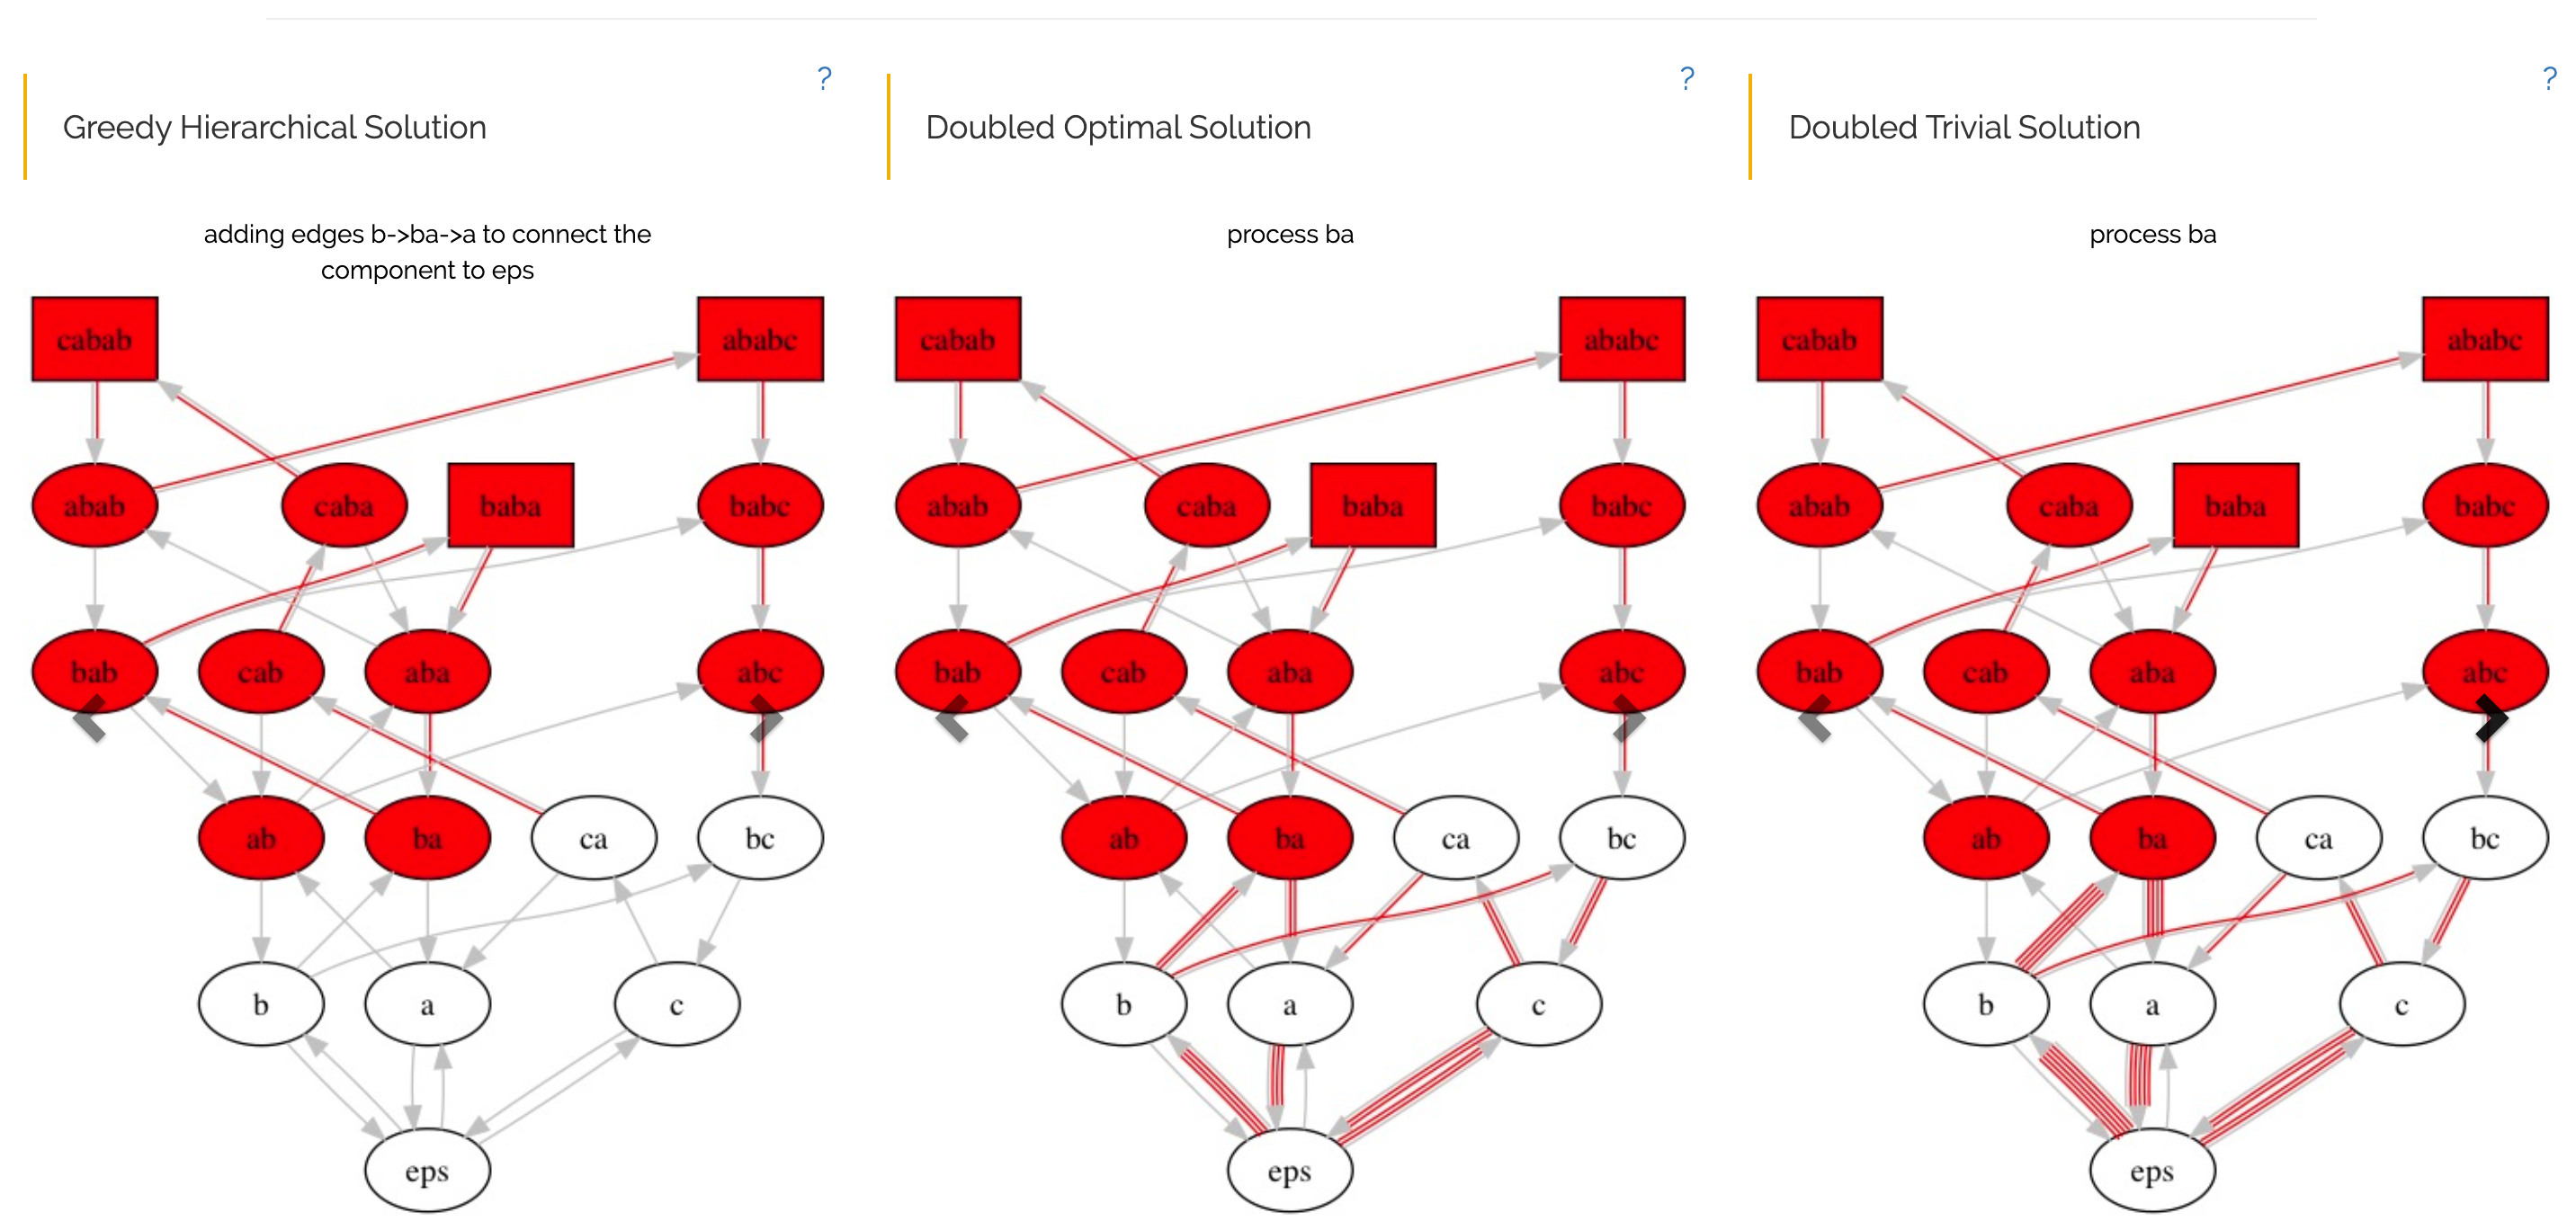
\includegraphics[width=\textwidth]{framework.png}
\end{frame}